\documentclass[11pt]{ekblite}
\newcommand\mtop{1in}
\newcommand\mbottom{1in}
\newcommand\mleft{1.2in}
\newcommand\mright{1.2in}
\usepackage[top=\mtop, bottom=\mbottom, left=\mleft, right=\mright]{geometry}

\newcommand{\comment}[1]{}
\newcommand\aaron[1]{\textcolor{red}{#1}}
\newcommand{\seay}[1]{\textcolor{blue}{#1}}
\hypersetup{ 	
pdfsubject = {Mathematics},
pdftitle = {fractal dimension},
pdfauthor = {Max Seay and Aaron Huntley}
}

\begin{document}

\title{Exploring fractal dimension\\
DRP spring 2025}
\maketitle
\begin{center}
Maxwell Seay and Aaron Huntley\\
\today
\end{center}

\tableofcontents

\newpage

\section{Preface}
This was written by Max Seay of CWRU with direction from PhD student Aaron Huntley, as part of the Directed Reading Program in Spring 2025. As of writing, it has not been proofread.

\newpage
\section{Introduction}
The goal is to find how to compute \textit{dimensionality}. I already know the \textit{dimensionality} of some things. I know the dimension of a point is 0, the dimension of a line is 1, the dimension of a square is 2, etc. But how is it calculated for some arbitrary object? In this case, by object, I mean:
\\[0.2in]A finite or infinite \textit{compact} set of points $x$, where $x \subset \R^n$.
\\[0.2in]Below are common examples of objects and their dimension.

\newpage
\section{How to measure the real numbers}
On the real number line a few common objects can be defined. For example:
\begin{example}[Point]
	A point on the real number line is a single real number. A point is a thing $x$ such that $x \in \R$. Examples include: $1,2,3,17,\sqrt{2},\pi$.
	\\[0.2in]The dimensionality of a point is commonly known to be 0. A point can't have length.
\end{example}
\begin{example}[Line segment]
	A line segment on the real number line is the defined to be the set of all real numbers that lie between two points. A line segment that starts at 0 and reaches 1 would be defined as the set
	\[\{x : 0 \le x \le 1\}\] 
	In other words, a set containing every real number between and including 0 and 1.
	\\[0.2in]A line segment is $\textit{closed}$ if it contains its end points. A line segment is $\textit{open}$ if it doesn't contain its end points.
	\\[0.2in]The dimensionality of a line is commonly known to be 1. And most line segments can be measured by finding the distance between the two points.  
	\\[0.2in]Line segments are also called $\textit{intervals}$.
\end{example}
\begin{example}[Finite set of points]
	A finite collection of points lying on the real number line. Only a single point alone has 0 dimensionality. Two points together also has 0 dimensionality. Combine any finite number of points and this combination will be 0 dimensional. A collection of 10 billion points is 0-dimensional, no matter what.
\end{example}
Is there a way to generalize this idea of measuring things on the real number line? Given any strange and arbitrary set of numbers, how should it be measured?

\begin{example}[Stick cutting]
	Let there be some stick $s$ to measure. Say the stick begins at a length of 1. Now do the following:
	\\[0.2in]Cut the stick to $\frac{1}{2}$ its original length. Then take the stick and cut it to $\frac{1}{3}$ its original length. Then cut the stick to $\frac{1}{4}$ its original length. Continue this forever. In the end how long is the resulting stick?
	\\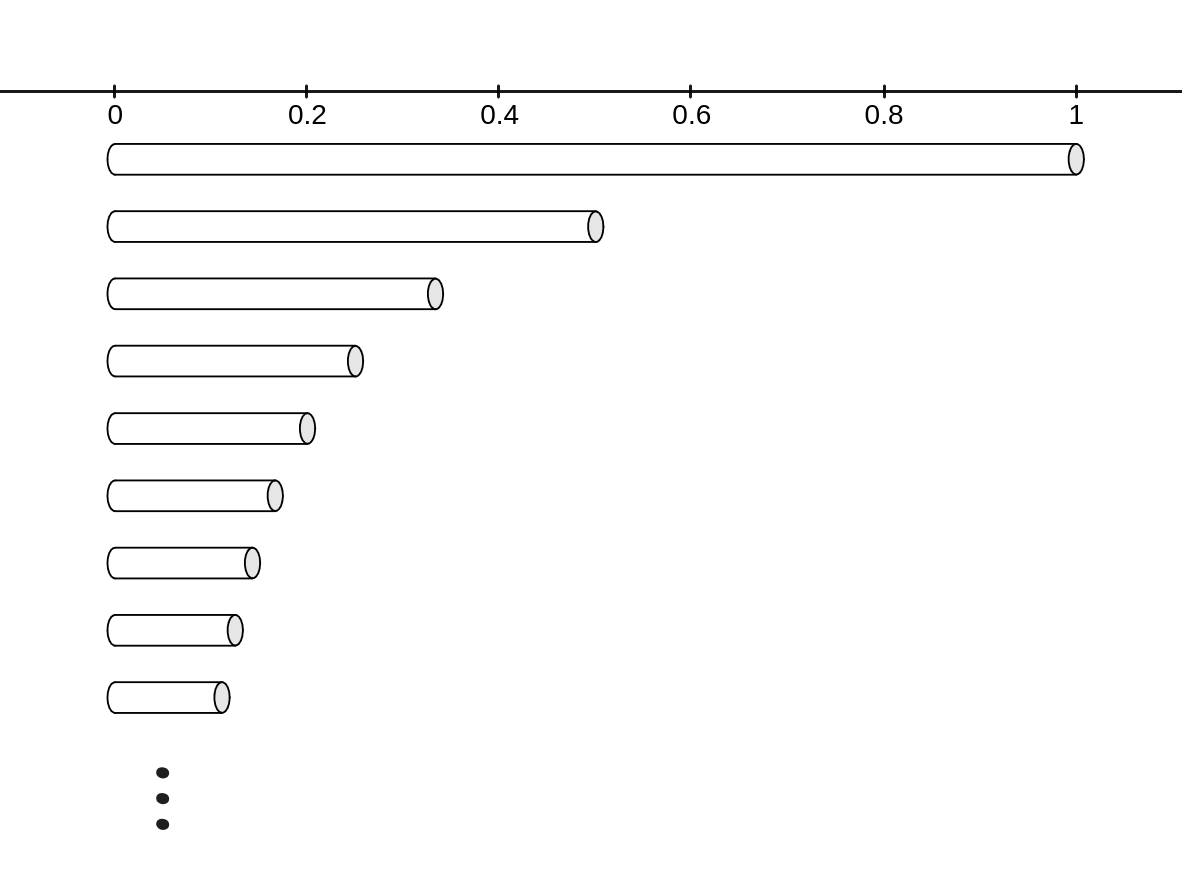
\includegraphics[scale=0.3]{img/c5.jpg}
	\\[0.2in]On one hand, the stick is cut forever, so it must be reduced to nothing by the end. On the other hand, the amount that gets cut off decreases each time and so at some point there may be no more cut off at all.
	\begin{corollary}
		The length of the stick after it's been through the cutting process is 0. 
	\end{corollary}
	To prove this, I will show that given any real number $\varepsilon$, the length of the stick is less than $\varepsilon$. Thus the length must be 0.
	\begin{proof}
		Let the stick be an interval (line segment). Let $s_0$ be the initial stick; a closed interval $[0,1]$.
		\\[0.2in]Step $1$ is to cut the interval in half. So the interval becomes $\left[0,\frac{1}{2}\right]$.
		\\[0.2in]Step $2$ is to cut the interval into a third. So the interval becomes $\left[0,\frac{1}{3}\right]$.
		\\[0.2in]Step $3$ is to cut the interval into a fourth. So the interval becomes $\left[0,\frac{1}{4}\right]$.
		\\[0.2in]Step $k$ is to cut the interval $\left[0,\frac{1}{k}\right]$ into the interval $\left[0,\frac{1}{k+1}\right]$.
		\\[0.2in]After every step of the cutting process, the stick is cut; the length of the interval is decreased. This can be seen by comparing the lengths of the stick before and after some cutting step $k$:
		\[\left| 0 - \frac{1}{k+1} \right| \le \left| 0 - \frac{1}{k} \right|\] 
		\\[0.2in]Let $\varepsilon \in \R^+$ be some arbitrary positive real number.
		\\[0.2in]I will show that there always exists a cutting step $k'$ such that after this step, the length of the stick is less than the arbitrarily small $\varepsilon$. 
		\\[0.2in]Choose the $k'$ step to be a whole number such that
		\[k' > \frac{1}{\varepsilon}\]
		(By the archimedian principle this is always possible.)
		\\[0.2in]I know that by definition of the cutting process, for this step $k'$, the stick is cut to a length $l$ that is
		\[l \le \frac{1}{k'}\] 
		And note that by the definition of $k'$ we have that
		\[l \le \frac{1}{k'} < \frac{1}{\sfrac{1}{\varepsilon}} = \varepsilon\]
		Or simply
		\[l < \epsilon\]
		Since the length of the stick $l$ at some step $k'$ is always less than $\varepsilon$, and $\varepsilon$ can be made arbitrarily small, it must be true that 
		\[l = 0\] 
		As required.
	\end{proof}
\end{example}

\subsection{Lebesgue measure}
A common way of measuring an object is to tighly cover it with something. The object's measure should be similar to that of the covering.
\\[0.2in]Like to measure the surface area of a sphere, tighly wrap a blanket around it so that it covers the sphere, then measure the blanket. This covering idea is often a part of definitions of measure and dimension.
\\[0.2in]In this case, (Lebesgue measure on the real number line), the covering is made from intervals. The covering of intervals tightly cover the object. The sum of the lengths of intervals is approximately the measure of the object itself.
\begin{definition}[Lebesgue measure]
	
\end{definition}

\newpage
\section{Notion of dimension: Minkowski–Bouligand or box-counting dimension}
I would like to know how to estimate the dimension of arbitrary objects. First I will look at simple examples to find out more about the notion of dimension.
\begin{example}[Line segment]
	I know what a line segment is. I also know every line segment is 1 dimensional.
	\\[0.2in]I take an approximation. I will cover a line segment with boxes. Each box has diameter (or radius) $r$. (To me it doesn't matter much since the difference between radius and diameter is always just a factor of 2.)
	\\[0.2in]Take the line segment to be the interval $[0,1]$. If $r = 1$, then I need only 1 box to cover the line segment.
	\\[0.2in]If $r = \sfrac{1}{2}$, I will need at least 2 boxes.
	\\[0.2in]If $r = \sfrac{1}{3}$, I will need at least 3 boxes.
	\\[0.2in]If $r = \sfrac{1}{n}$, I will need at least $n$ boxes to cover the line segment.
	\\[0.2in]I will define a function that takes in a radius, $r$, and outputs the least number of boxes of radius $r$ needed to cover the line segment. From the above examples it can be seen that this function is:
	\[\mathcal{N}(r) = \frac{1}{r}\]
	Another idea to think on. How to double the \textit{length} of the line segment? To double the length of the line segment, copy and paste it once, and append the copy onto the end of the original. 
	\\[0.2in]So in other words, to double the length of the line segment, add 1, (or $2^1 - 1$ you could say,) extra copy.
\end{example}
\begin{example}[Square]
	I know what a square is. I also know every square is 2 dimensional.
	\\[0.2in]I take an approximation. I will cover a square with boxes. Each box has diameter (or radius) $r$.
	\\[0.2in]Take the square to be the unit square, $[0,1] \times [0,1]$. If $r = 1$, then I need only 1 box to cover the square. (The box and square are the same.)
	\\[0.2in]If $r = \sfrac{1}{2}$, I will need at least 4 boxes.
	\\[0.2in]If $r = \sfrac{1}{3}$, I will need at least 9 boxes.
	\\[0.2in]If $r = \sfrac{1}{n}$, I will need at least $n^2$ boxes to cover the unit square.
	\\[0.2in]I will define a function that takes in a radius, $r$, and outputs the least number of boxes of radius $r$ needed to cover the square. From the above examples it can be seen that this function is:
	\[\mathcal{N}(r) = \frac{1}{r^2}\]
	Now how to double the \textit{area} of the square? To double the area of the square, copy and paste it three times, and append the copies to three sides of the original. 
	\\[0.2in]So in other words, to double the area of the square, add 3, (or $2^2 - 1$ you could say,) extra copies.
\end{example}
So for the line segment we have that the number of squares of radius $r$ needed to cover it as
\[\mathcal{N}(r) = \frac{1}{r}\]
And for the square we have that the number of squares of radius $r$ needed to cover it as
\[\mathcal{N}(r) = \frac{1}{r^2}\]
From these couple examples it seems that, in general
\[\mathcal{N}(r) = c \left(\frac{1}{r}\right)^d\]
Where $c$ is a constant. It seems that it would be appropriate to call the $d$ in this expression the dimension. This function $\mathcal{N}(r)$ is called a power law since $\sfrac{1}{r}$ is always raised to some power. \cite{falconer2}

\newpage
\section{Notion of Dimension: Hausdorff measure and dimension}
\newpage
\section{Cantor Set}
	Let $\mathcal{C}$ be the Cantor Set.
	\begin{definition}[Cantor Set]
        $\mathcal{C}$ can be described as an intersection of an infinite sequence of sets. The sequence of sets, $\{\mathcal{C}_i\}_{i=0}^{\infty}$, is defined recursively. For example, the first three are:
		\[C_0 = [0,1]\]
		\[C_1 = \left[0,\sfrac{1}{3}  \right] \cup \left[ \sfrac{2}{3},1\right]\]
		\[C_2 = \left[0,\sfrac{1}{9}  \right] \cup \left[ \sfrac{2}{9},\sfrac{3}{9} \right] \cup \left[\sfrac{6}{9},\sfrac{7}{9}\right] \cup \left[ \sfrac{8}{9},1\right]\]
		\[C_3 = \left[0,\sfrac{1}{27}  \right] \cup \left[\sfrac{2}{27},\sfrac{3}{27}  \right] \cup \left[\sfrac{6}{27},\sfrac{7}{27}  \right] \cup \left[\sfrac{8}{27},\sfrac{9}{27}  \right] \cup \left[\sfrac{18}{27},\sfrac{19}{27}  \right] \cup \left[\sfrac{20}{27},\sfrac{21}{27}  \right] \cup \left[\sfrac{24}{27},\sfrac{25}{27}  \right] \cup \left[\sfrac{26}{27},1  \right]\]
		\\
		And the recursive definition for a set $\mathcal{C}_i$ is:
		\[\mathcal{C}_i = \frac{1}{3} \mathcal{C}_{i-1} \cup \frac{2}{3} + \frac{1}{3} \mathcal{C}_{i-1}\]
	\end{definition}
	\begin{corollary}
		$\mathcal{C}_i \ne \mathcal{C}$ for all $i \in \mathbb{N}$. No set in the sequence $\{\mathcal{C}_i\}$ is the Cantor Set, however the further you go (the larger the $i$), the ``closer'' $\mathcal{C}_i$ becomes $\mathcal{C}$. 
	\end{corollary}
	\begin{corollary}
		If $x \notin [0,1]$, then $x \notin \mathcal{C}$.
	\end{corollary}
	\begin{corollary}
		The Cantor Set is non-empty.
	\end{corollary}
	\begin{proof}Consider the point 0.
	\\[0.2in]$0 \in [0,1]$ so $0 \in \mathcal{C}_0$.
	\\[0.2in]Now make the assumption that $0 \in \mathcal{C}_k$.
	\\[0.2in]And since $\frac{1}{3} \cdot 0 = 0$ it must be true that
	\[0 \in \frac{1}{3} \cdot \mathcal{C}_k\] 
	\\[0.2in]Note that by definition we have that
	\[\mathcal{C}_{k+1} = \frac{1}{3} \mathcal{C}_{k} \cup \frac{2}{3} + \frac{1}{3} \mathcal{C}_{k}\]
	Well since $0 \in \frac{1}{3} \cdot \mathcal{C}_k$ it must be true that
	\[0 \in \frac{1}{3} \mathcal{C}_{k} \cup \frac{2}{3} + \frac{1}{3} \mathcal{C}_{k}\]
	or
	\[0 \in \mathcal{C}_{k+1}\]
	So by induction we have that
	\[0 \in \mathcal{C}\]
	Thus $\mathcal{C}$ is non-empty.
	\end{proof}
	\begin{corollary}
		The Cantor Set is a proper subset of $[0,1]$.
	\end{corollary}
	\begin{corollary}
		$\mathcal{C}_{i}$ is always a covering of $\mathcal{C}_{i+1}$ and also always a covering of $\mathcal{C}$.
	\end{corollary}
	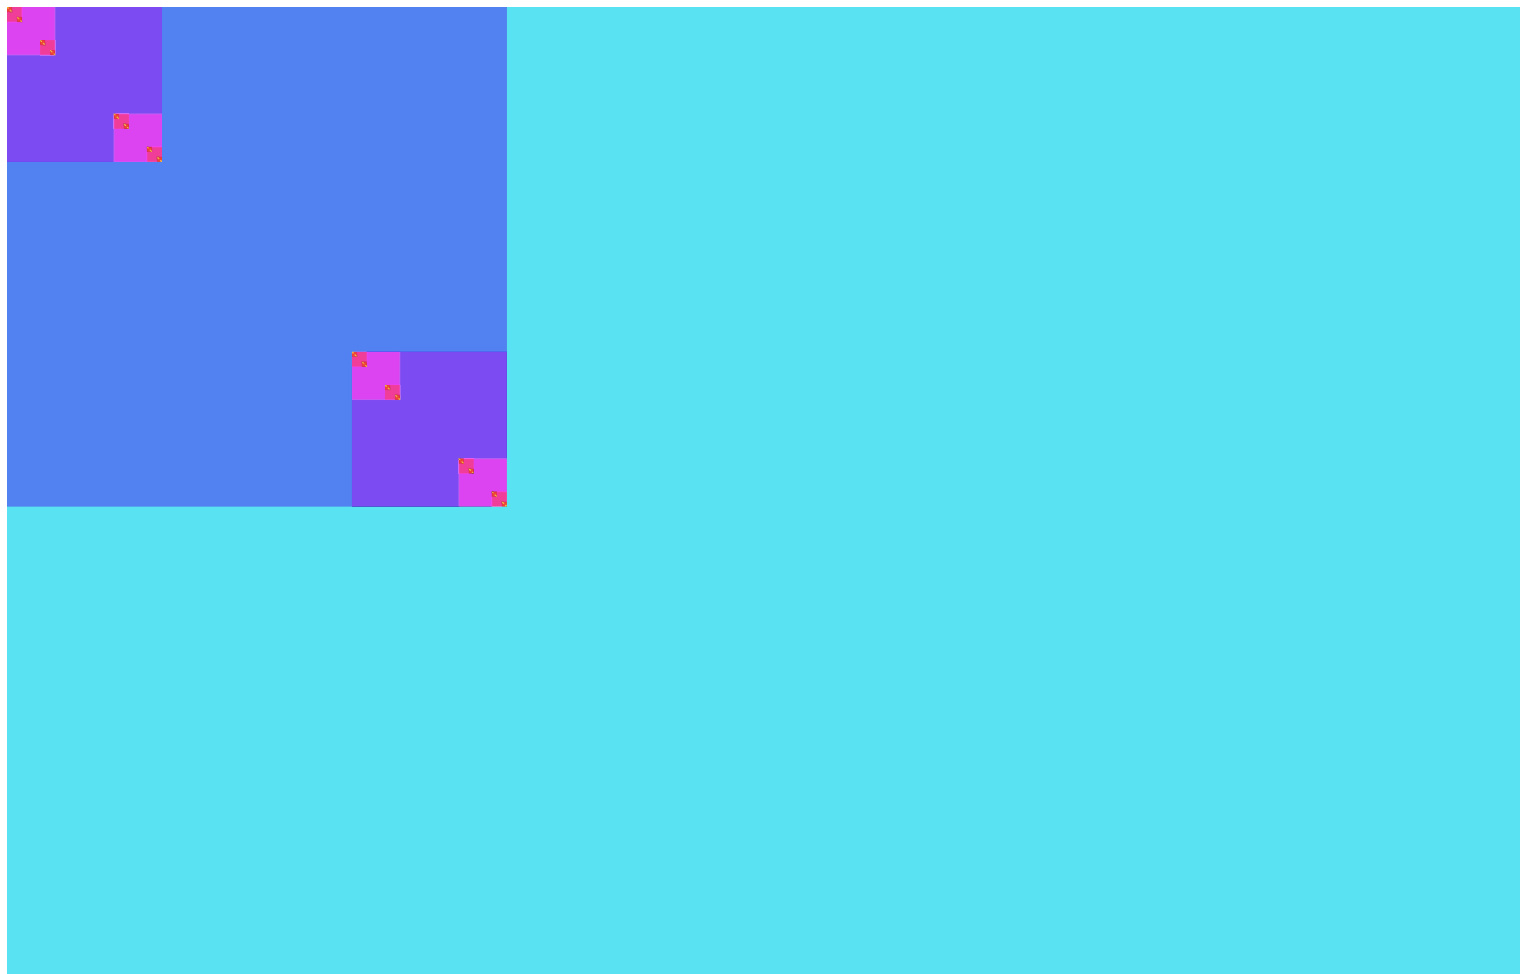
\includegraphics[scale=0.2]{img/c1.jpg}
	\\Cantor Set visualized in 2D with 10 iterations. For each interval $[a,b]$ of the set, there is a colored box positioned at $(a,a)$ with size $(3^{-k}, 3^{-k})$, where $k$ is the iteration. 
	\\[0.2in]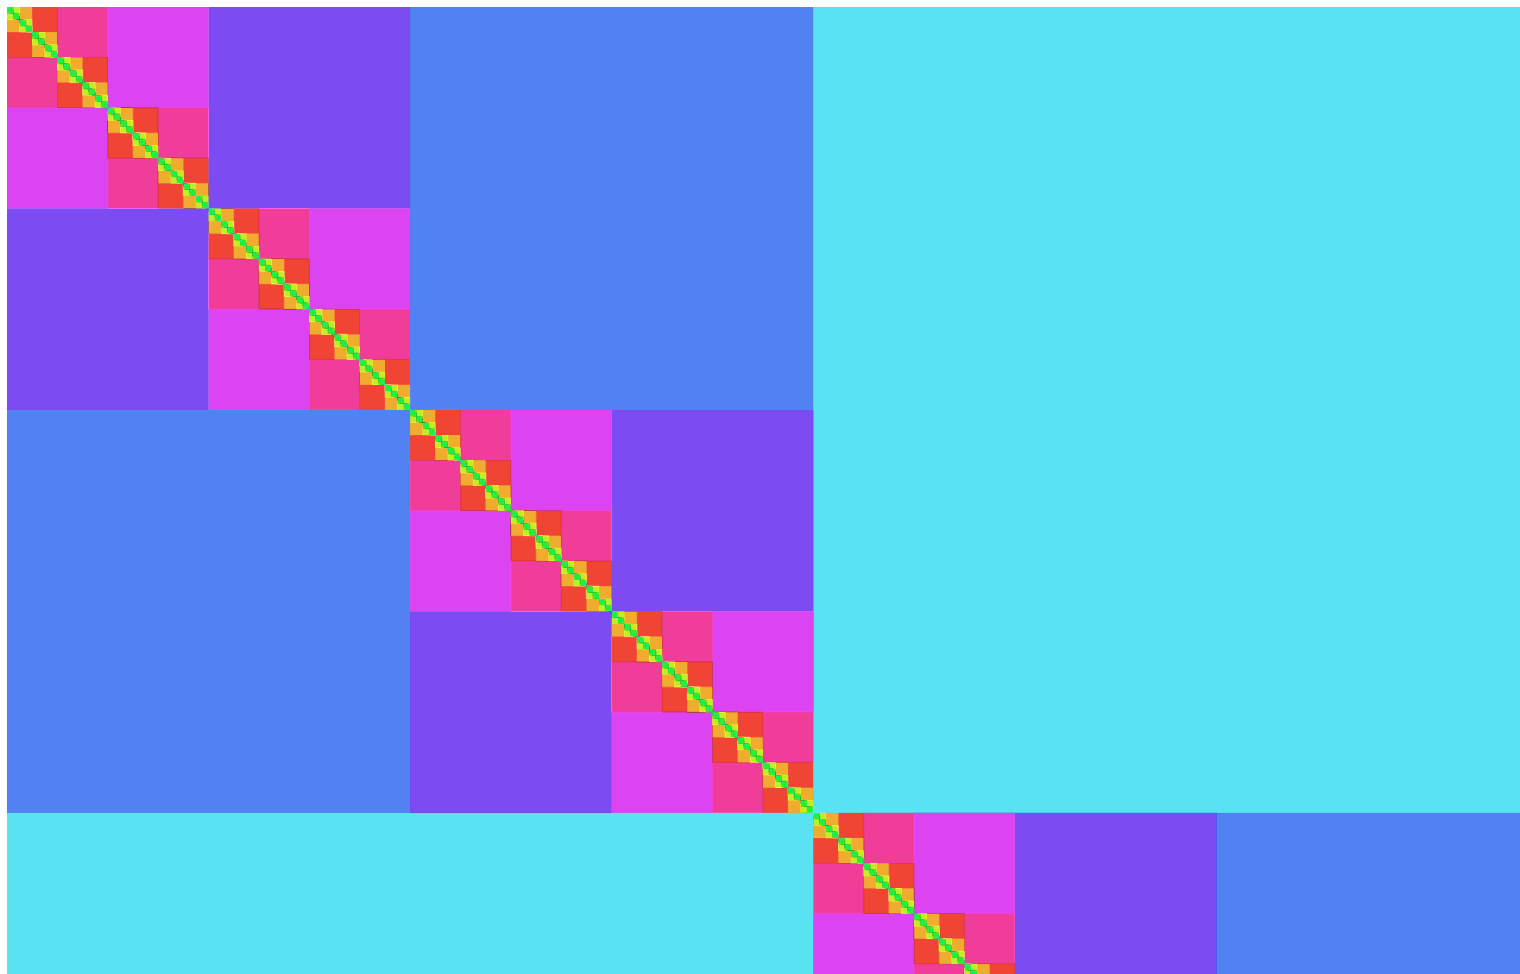
\includegraphics[scale=0.2]{img/c2.jpg}
	\\A set visualized in 2D with 10 iterations constructed the same way as the Cantor Set. However the $\frac{1}{3}$ in the Cantor Set definition is replaced with $\frac{1}{2}$ instead. 
	\\[0.2in]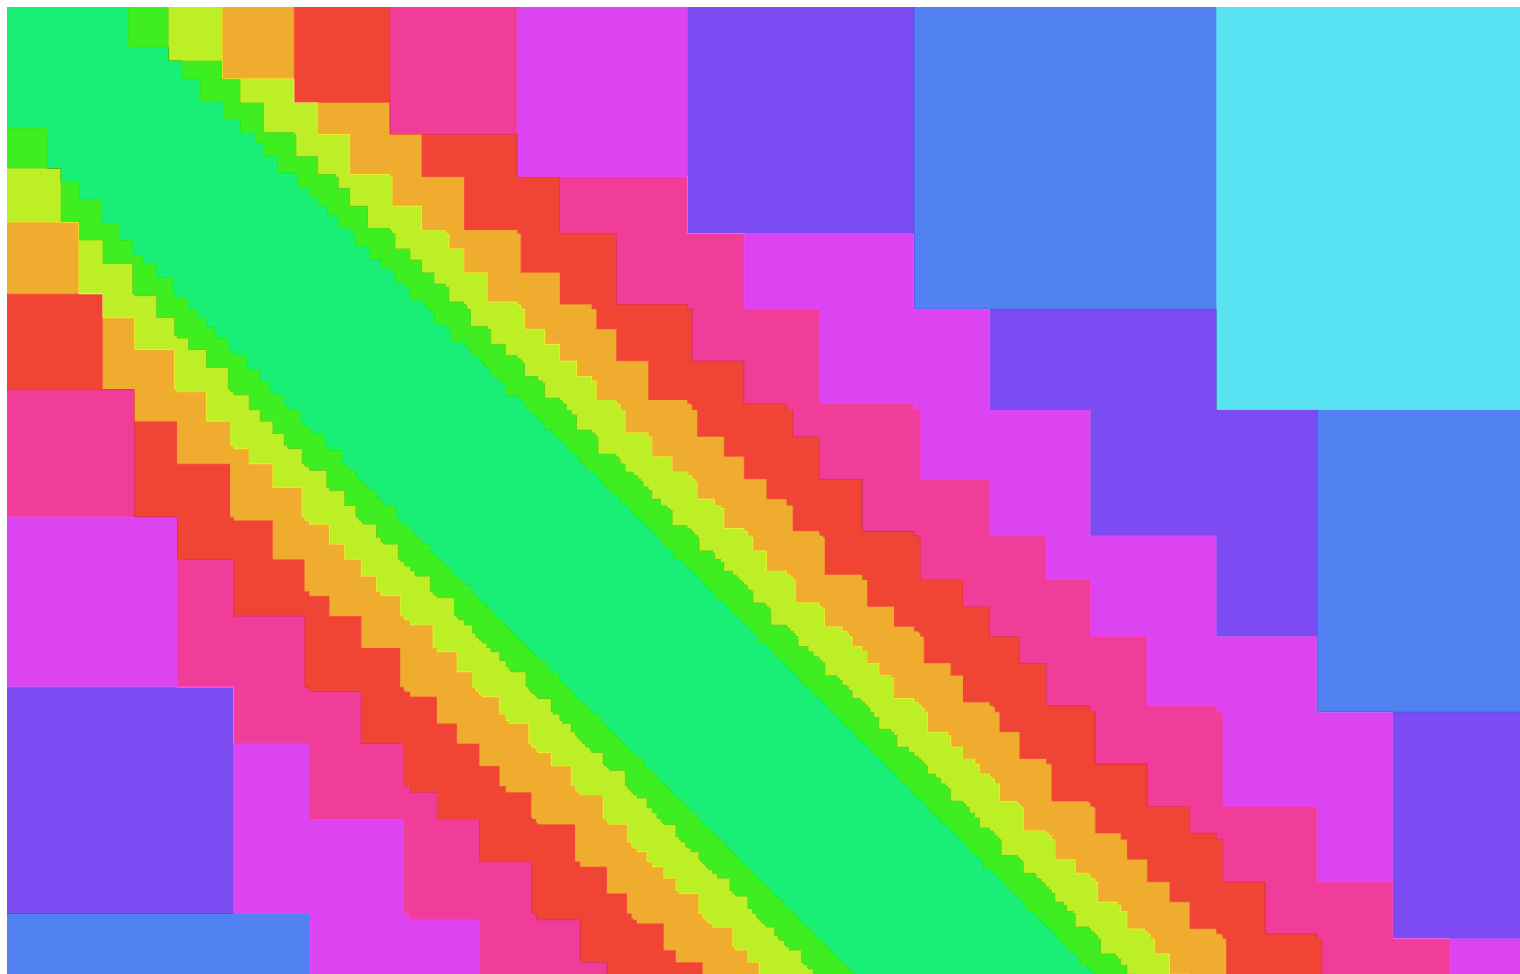
\includegraphics[scale=0.2]{img/c3.jpg}
	\\A set visualized in 2D with 10 iterations constructed the same way as the Cantor Set. However the $\frac{1}{3}$ in the Cantor Set definition is replaced with $\frac{3}{4}$ instead. 
	\\[0.2in]
\includegraphics[scale=0.2]{img/c4.jpg}
	\\A set visualized in 2D with 10 iterations constructed the same way as the Cantor Set. However the $\frac{1}{3}$ in the Cantor Set definition is replaced with $\frac{4}{5}$ instead. 
\newpage
\section{Dragon}

\newpage
\bibliography{citations}

\end{document}
